\section{Diagrammi di attività}

Vengono in seguito illustrati i diagrammi di attività prodotti durante la progettazione architetturale, i quali descrivono le iterazioni dell'utente con il sistema \glossario{MaaP}. È stato scelto di dividere i diagrammi in due categorie principali, in modo analogo a quanto fatto nella descrizione dei casi d'uso dell'\textit{Analisi dei requisiti}:

\begin{itemize}

	\item \textbf{Applicazione \glossario{MaaP}}, in cui verranno descritte le iterazioni che un utente può fare all'interno di un'applicazione generata dal \glossario{framework};
	\item \textbf{Servizio \glossario{MaaS}}, in cui verranno descritte le iterazioni all'interno del suddetto servizio web.

\end{itemize}
Inizialmente per ogni categoria verrà fornito uno schema ad alto livello, per poi andare sempre più nel dettaglio tramite sotto-diagrammi più specifici. Per comodità di visualizzazione le attività che verranno \textit{esplose} sono marcate in grassetto. 

Al fine di rendere il diagramma leggibile abbiamo considerato implicito il fatto che un utente possa in qualsiasi momento uscire dall'applicazione \glossario{MaaP} o dal servizio \glossario{MaaS}, per esempio chiudendo la finestra del browser.

\subsection{Applicazione MaaP}

Vengono di seguito descritte tutte le iterazioni che un utente può effettuare con un'applicazione generata dal \glossario{framework} \glossario{MaaP}.


\subsubsection{Attività principali}

\begin{figure}[H]
\centering
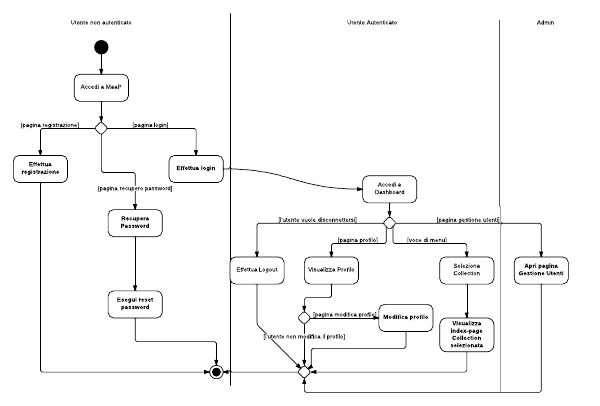
\includegraphics[scale=0.7]{uml/MaaP - Attivita principali.png}
\caption{Diagramma di attività - Attività principali di un'applicazione MaaP}
\end{figure}

Sostanzialmente un'applicazione generata da \glossario{MaaP} è composta da una serie di pagine web all'interno delle quali un utente può navigare. Un utente accede inizialmente all'applicazione web in una pagina statica in cui può effettuare tre cose:

\begin{itemize}

	\item Registrarsi al sistema;
	\item Effettuare il login;
	\item Recuperare la propria password.

\end{itemize}

Una volta che l'utente ha effettuato il login viene direttamente indirizzato alla \glossario{Dashboard}, dalla quale può navigare all'interno dell'applicazione ed effettuare diverse operazioni:

\begin{itemize}

	\item Effettuare il logout;
	\item Visualizzare il proprio profilo e di conseguenza modificarlo;
	\item Selezionare una \glossario{Collection} esistente.

\end{itemize}

Nel caso in cui l'utente avesse i privilegi di admin può inoltre accedere ad una specifica pagina di gestione degli utenti iscritti.

\subsubsection{Effettua registrazione}

\begin{figure}[H]
\centering
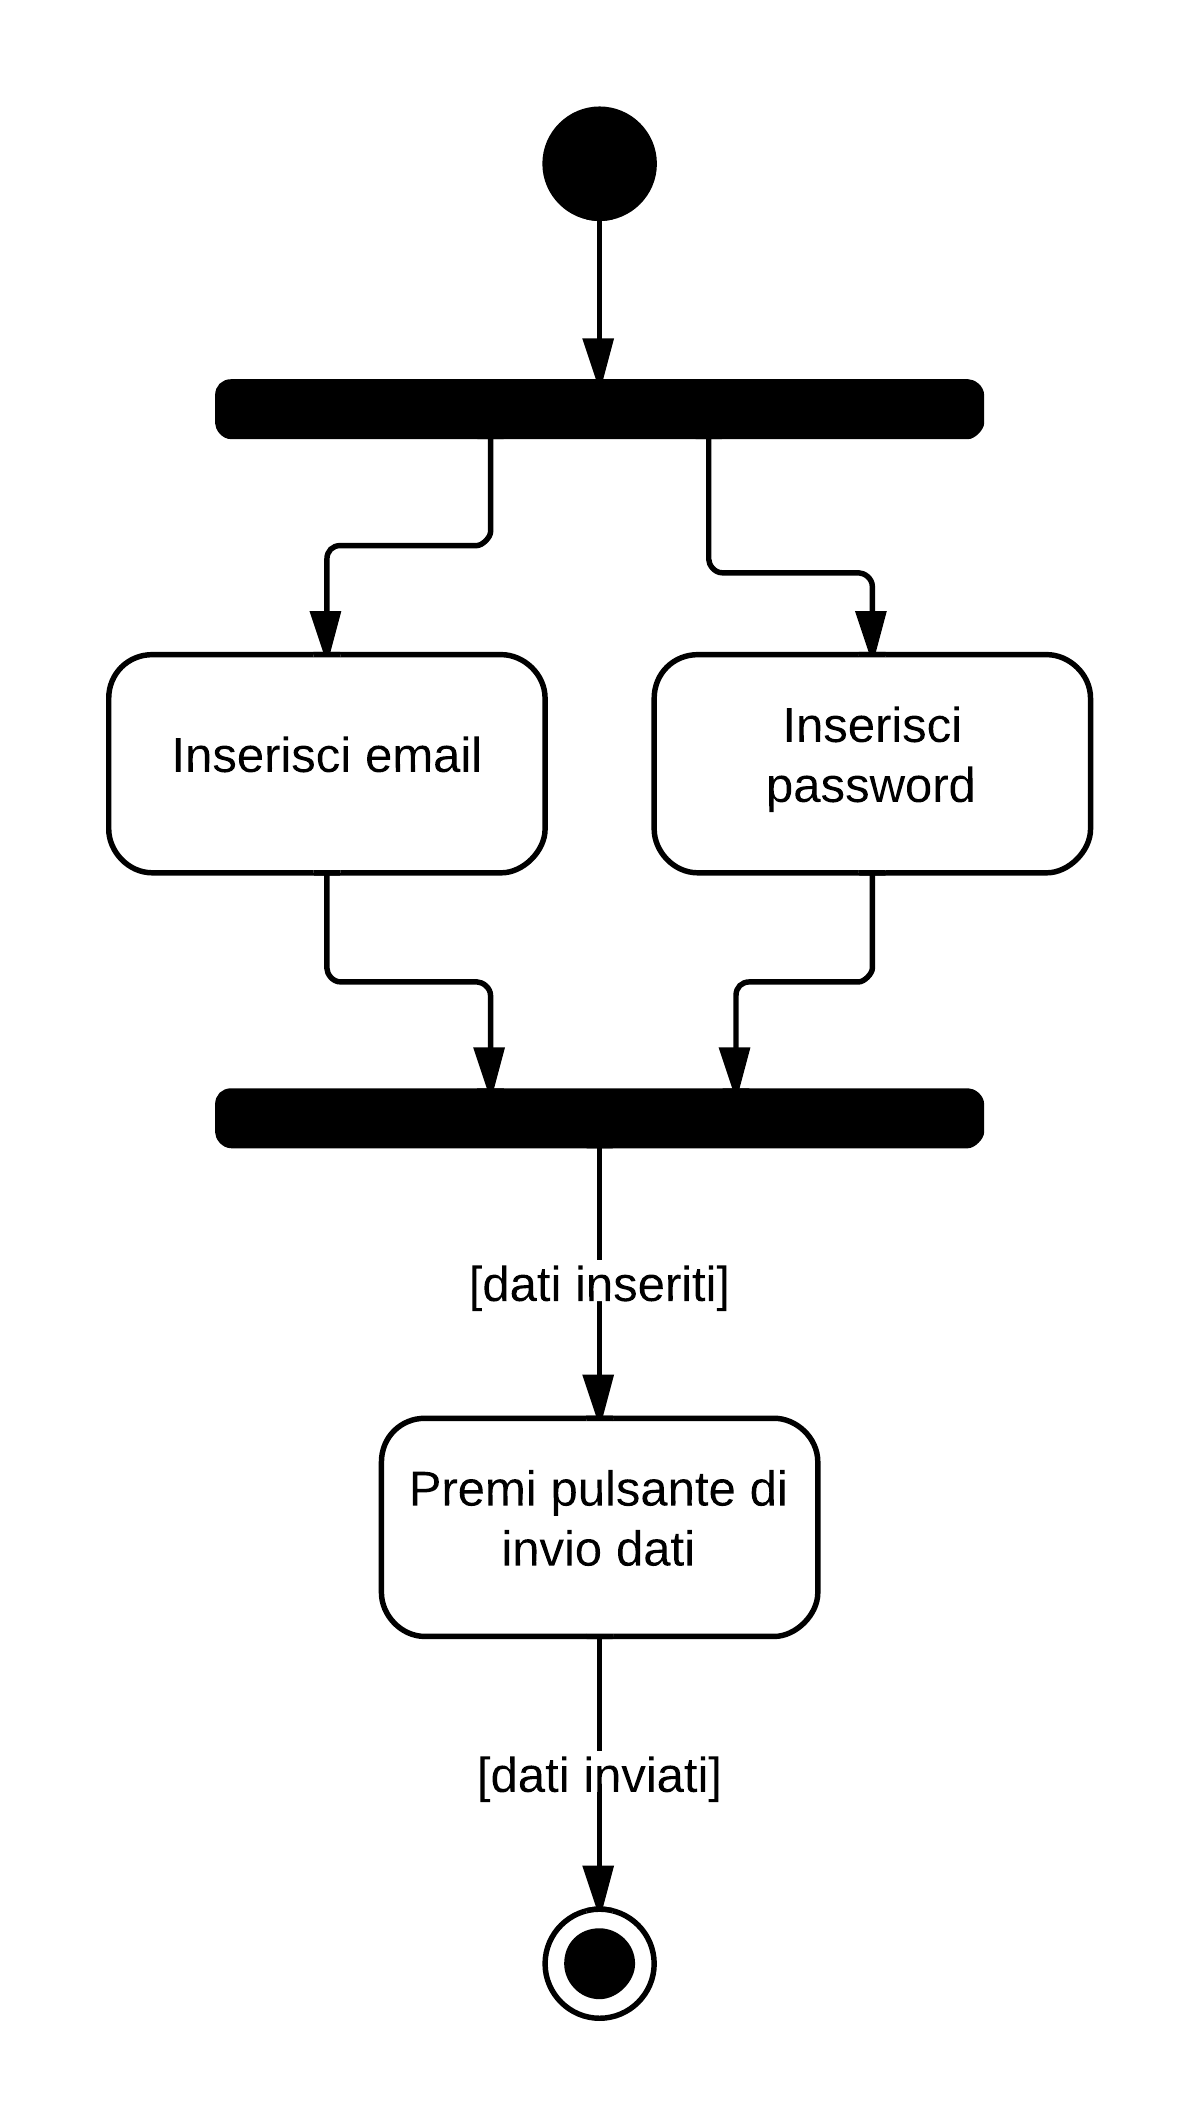
\includegraphics[scale=0.2]{uml/MaaP - Effettua registrazione.png}
\caption{Diagramma di attività - Registrazione di un utente}
\end{figure}

L'utente si trova all'interno della pagina di registrazione e sostanzialmente deve inserire la propria email e la propria password all'interno di due campi di testo. Una volta inseriti l'utente deve premere il pulsante di invio dati; il sistema \glossario{MaaP} procederà dunque alla verifica delle credenziali e, se quest'ultima avrà successo, alla registrazione dell'utente.

\subsubsection{Recupera password}

\begin{figure}[H]
\centering
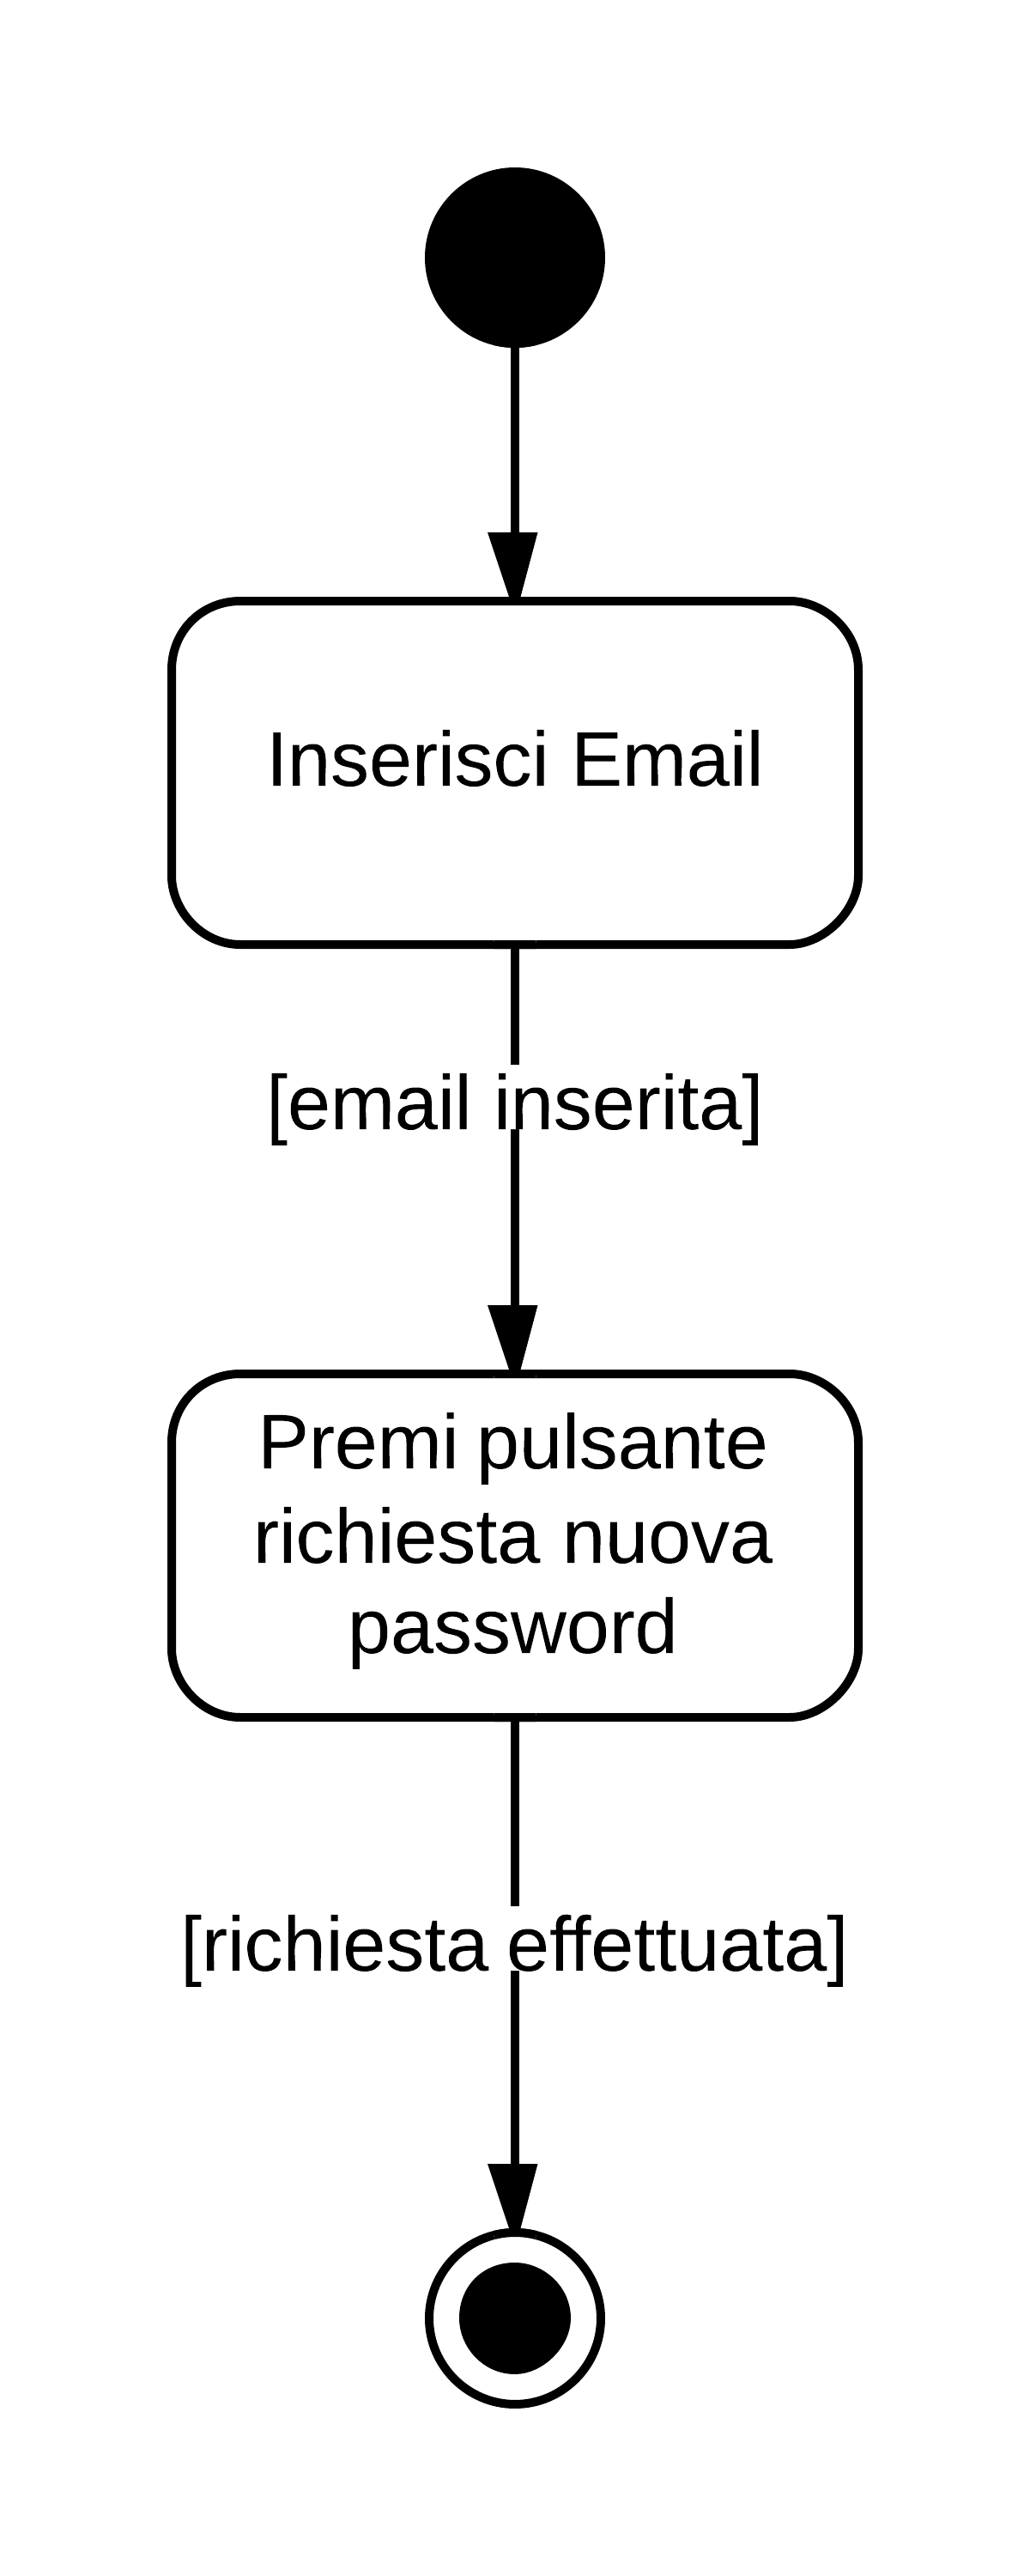
\includegraphics[scale=0.1]{uml/MaaP - Recupera password.png}
\caption{Diagramma di attività - Recupero password}
\end{figure}

L'utente si trova all'interno della pagina di recupero password, la quale presenta un campo di testo nel quale l'utente dovrà inserire il proprio indirizzo email. Una volta inserito preme il pulsante di richiesta di una nuova password; il sistema \glossario{MaaP} procederà dunque alla verifica dell'indirizzo email e, se quest'ultima avrà esito positivo, invierà un'email all'utente con le relative istruzioni per il ripristino della password.

\subsubsection{Esegui reset password}

\begin{figure}[H]
\centering
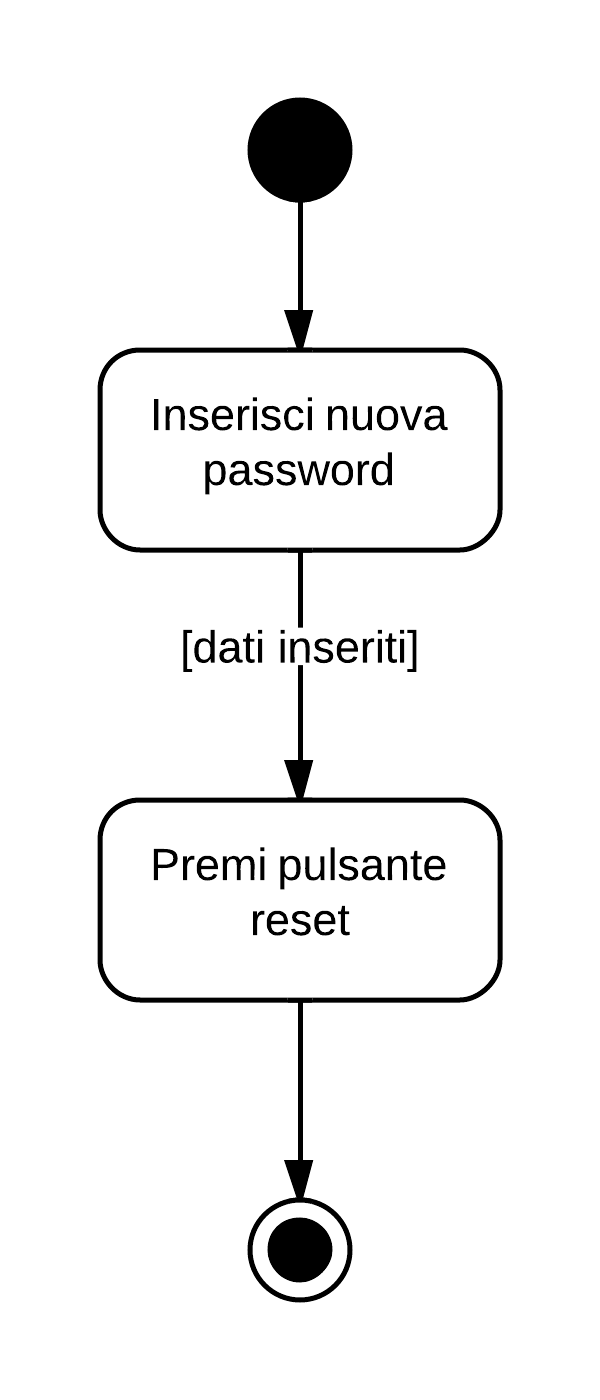
\includegraphics[scale=0.1]{uml/MaaP - Esegui reset password.png}
\caption{Diagramma di attività - Reset della password dell'utente}
\end{figure}

L'utente avrà ricevuto un'email con al suo interno un link ad una pagina univoca dell'applicazione \glossario{MaaP} e quindi si troverà in una pagina con al suo interno un campo di testo nel quale inserire la nuova password. Una volta inserita la password deve premere il pulsante di reset; il sistema \glossario{MaaP} procederà dunque al cambio password per l'utente corrente nel \glossario{database} delle credenziali.

\subsubsection{Effettua login}

\begin{figure}[H]
\centering
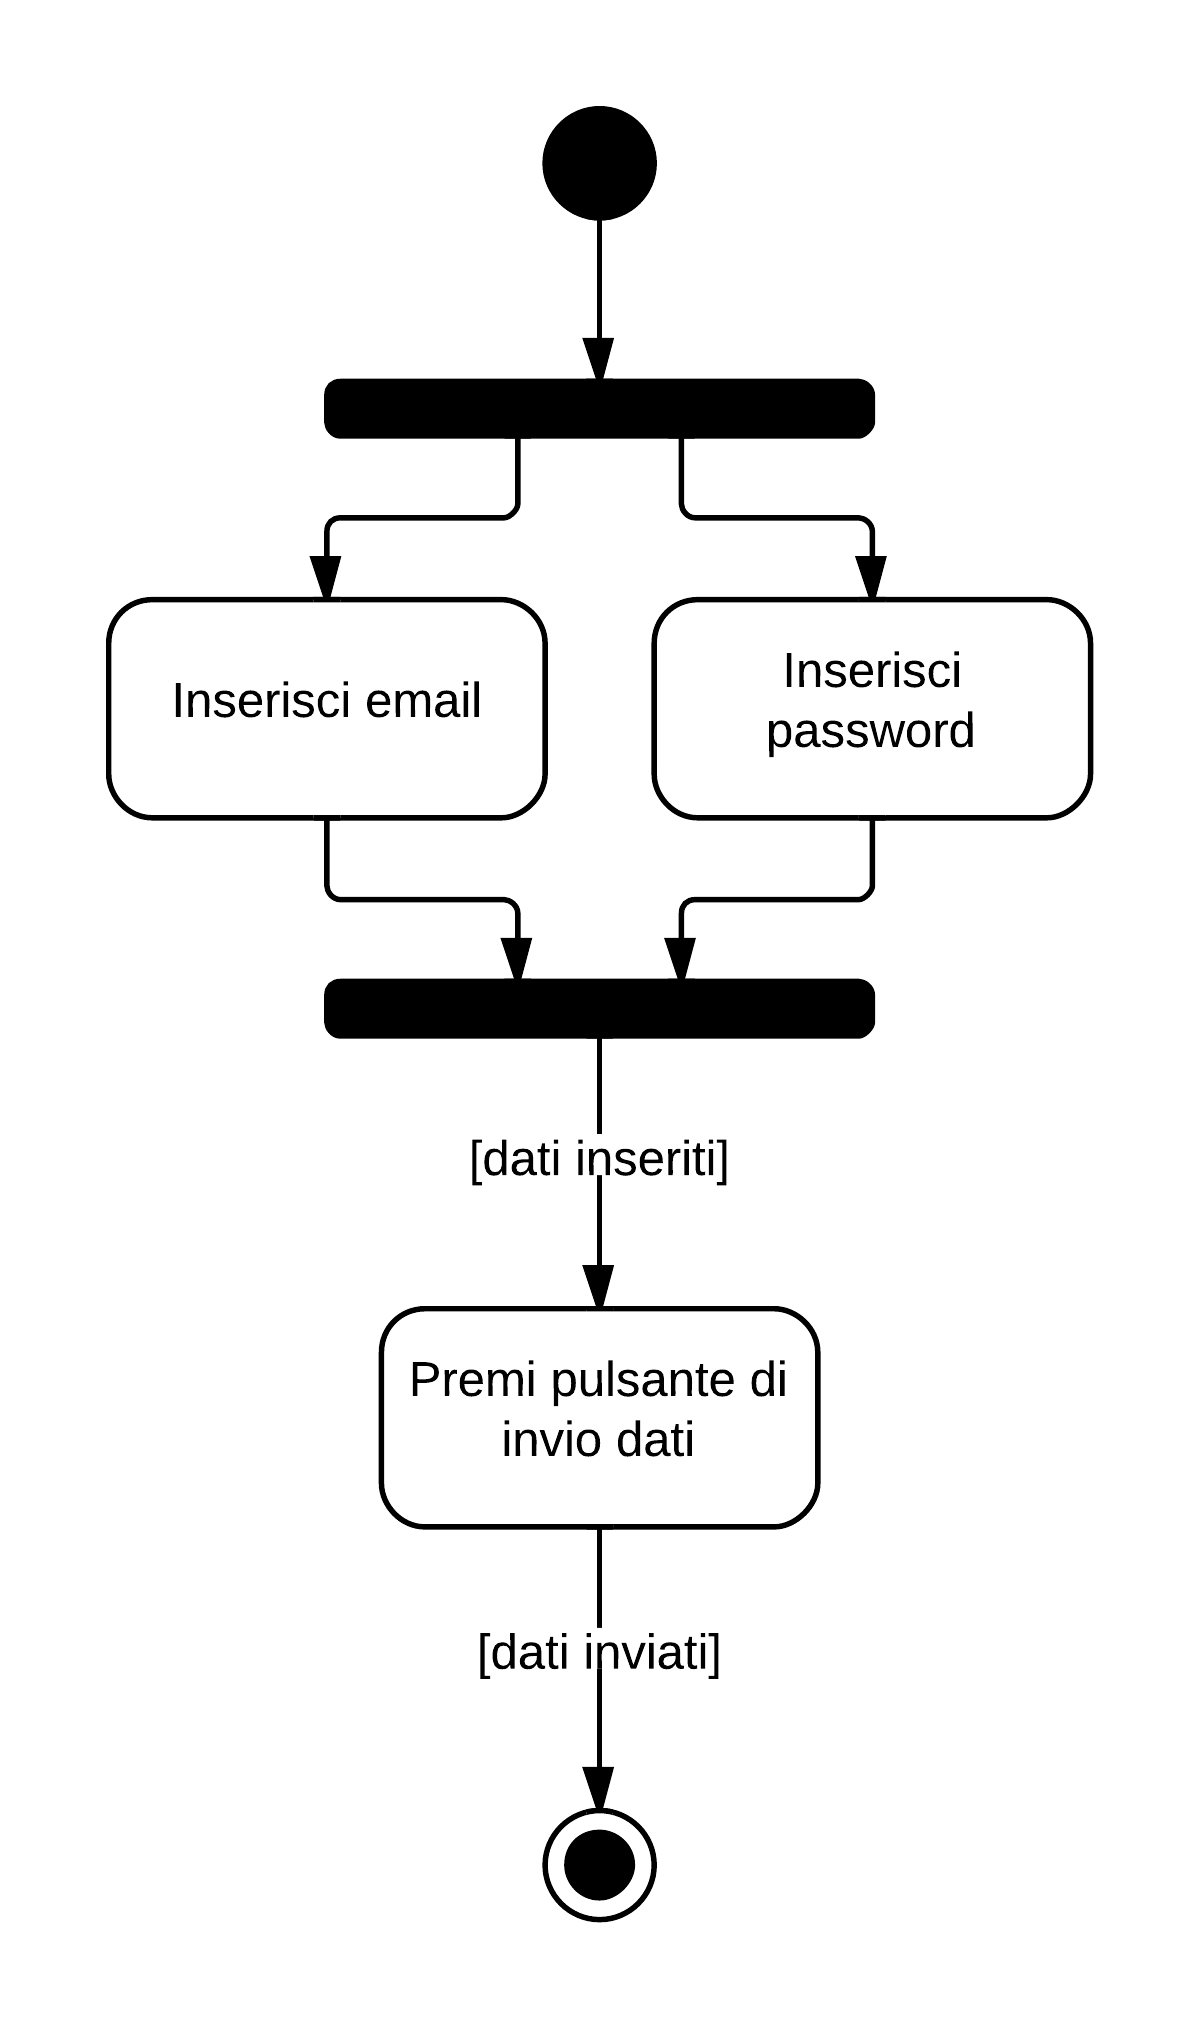
\includegraphics[scale=0.2]{uml/MaaP - Effettua login.png}
\caption{Diagramma di attività - Login dell'utente}
\end{figure}

L'utente, che precedentemente avrà effettuato la registrazione al sistema, accede all'interno dell'applicazione tramite una pagina di login. Al suo interno saranno presenti due campi di testo in cui l'utente dovrà inserire la propria email e la propria password. Una volta inserite dovrà premere il pulsante di login; il sistema \glossario{MaaP} procederà dunque alla verifica delle credenziali e, se l'esito di tale verifica risulterà positivo, effettuerà il login dell'utente all'applicazione, reindirizzandolo alla \glossario{dashboard}.

\subsubsection{Modifica profilo}

\begin{figure}[H]
\centering
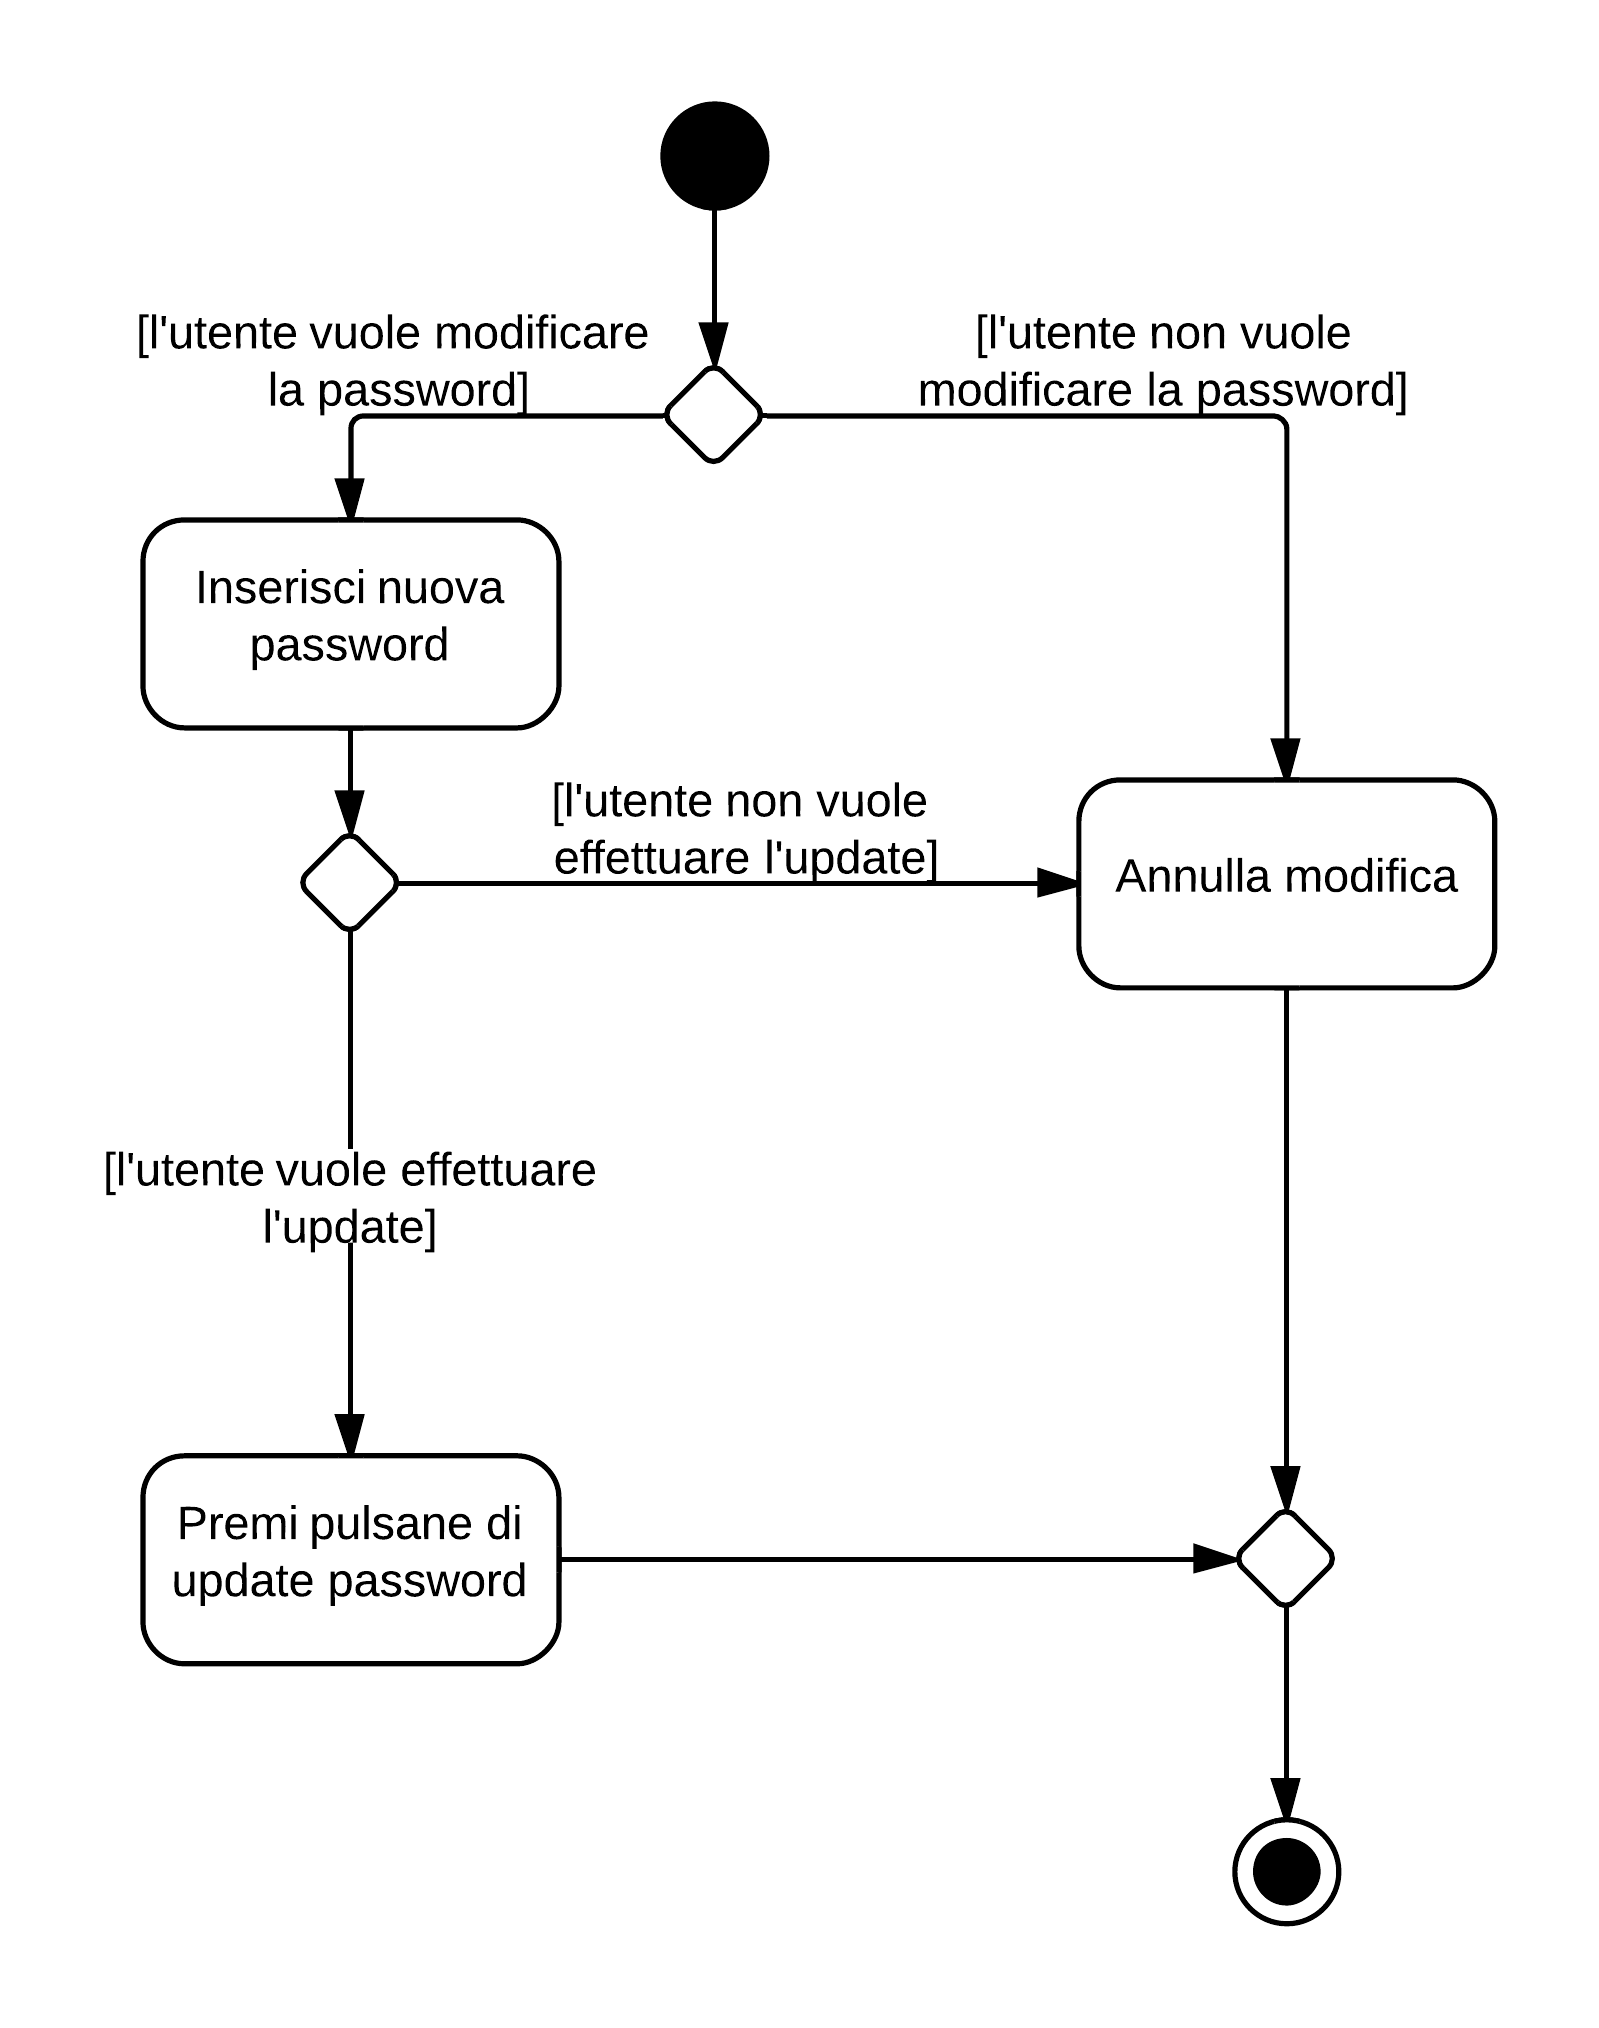
\includegraphics[scale=0.3]{uml/MaaP - Modifica profilo.png}
\caption{Diagramma di attività - Modifica profilo utente}
\end{figure}

L'utente autenticato accede all'interno della propria pagina profilo, dalla quale può decidere di modificare la propria password. Sarà dunque presente un campo di testo in cui l'utente inserirà la nuova password e un bottone tramite il quale invierà la richiesta di modifica; il sistema \glossario{MaaP} procederà dunque alla modifica della password dell'utente. L'utente in ogni momento può decidere di annullare le modifiche e tornare alla pagina precedente.

\subsubsection{Index-page Collection}

\begin{figure}[H]
\centering
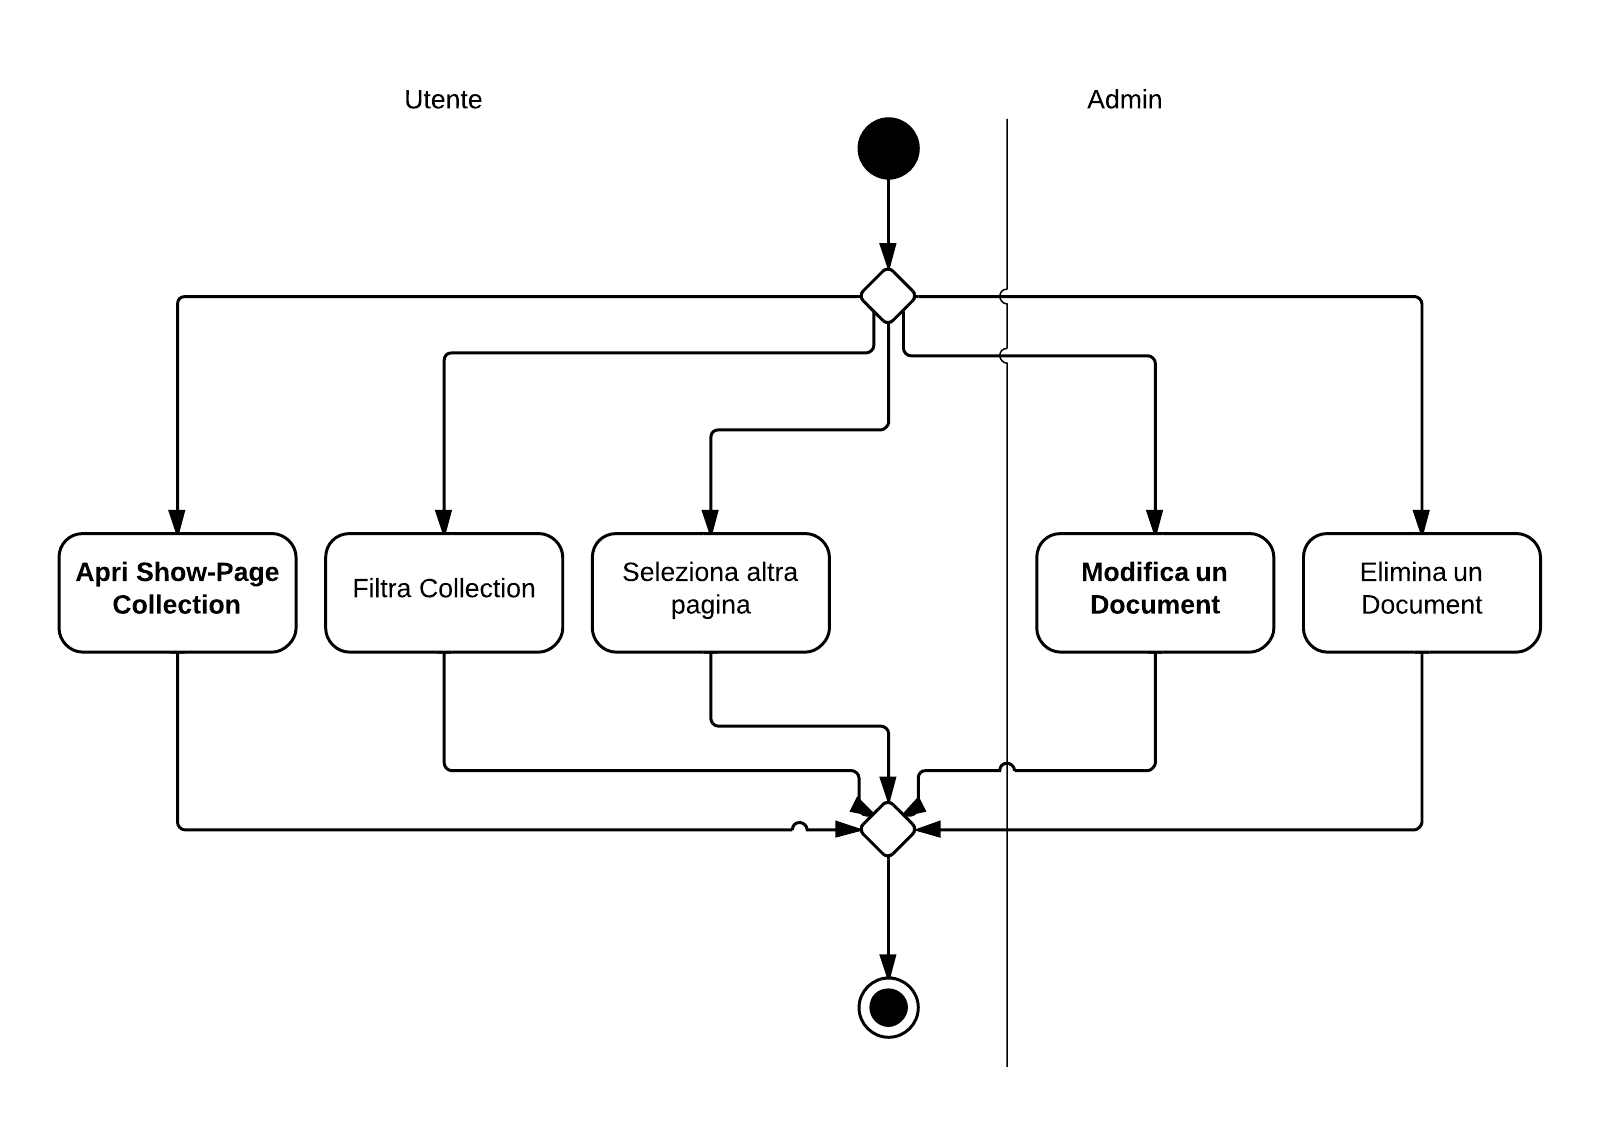
\includegraphics[scale=0.5]{uml/MaaP - Index-page.png}
\caption{Diagramma di attività - Visualizzazione index-page della Collection selezionata}
\end{figure}

L'utente ha selezionato una \glossario{Collection} dal menu e ora si trova all'interno di una pagina che visualizza una tabella contenente tutti i \glossario{Document} della \glossario{Collection} con alcuni attributi visualizzabili. A questo punto è in grado di fare diverse operazioni:

\begin{itemize}

	\item Può aprire la relativa \glossario{show-page} di un \glossario{Document} selezionando il link che la apre;
	\item Può applicare un filtro ai \glossario{Document} visualizzati in modo da visualizzare un sottoinsieme della tabella;
	\item Se la tabella risulta distribuita su più pagine può accedere alle pagine successive;

\end{itemize}

Se l'utente dispone dei privilegi di admin può inoltre:

\begin{itemize}

	\item Modificare un \glossario{Document} cliccando sul link \textit{edit} visualizzato in ciascuna riga della tabella;
	\item Eliminare un \glossario{Document} cliccando sul link \textit{delete} visualizzato in ciascuna riga della tabella;

\end{itemize}

\subsubsection{Show-page Document}

\begin{figure}[H]
\centering
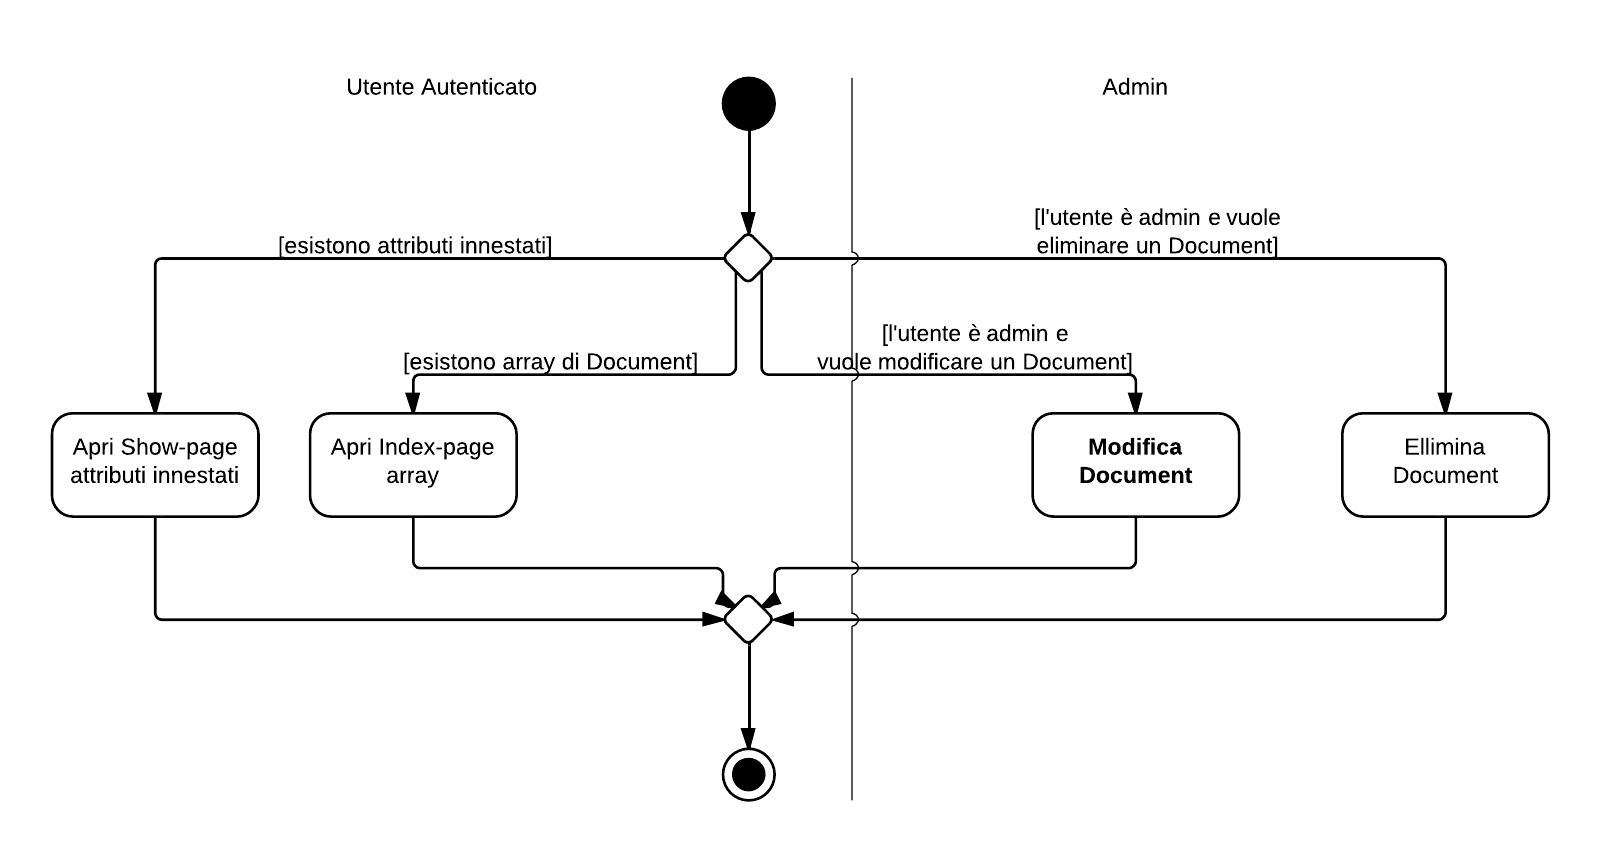
\includegraphics[scale=0.5]{uml/MaaP - Show-page.png}
\caption{Diagramma di attività - Visualizzazione show-page del Document selezionato}
\end{figure}

L'utente ha selezionato un \glossario{Document} dalla \glossario{index-page} e ora si trova davanti una pagina di visualizzazione dettagliata del \glossario{Document} selezionato. Sostanzialmente questa pagina conterrà una tabella contenente gli attributi visualizzabili del \glossario{Document}. Un utente all'interno di questa pagina può:

\begin{itemize}

	\item Aprire la \glossario{show-page} di un attributo innestato, se ne esiste uno;
	\item Aprire la \glossario{index-page} di un array di \glossario{Document}, se ne esiste uno.

\end{itemize}

Se l'utente possiede i privilegi di admin può inoltre:

\begin{itemize}

	\item Modificare gli attributi del \glossario{Document};
	\item Eliminare il \glossario{Document} corrente.

\end{itemize}

\subsubsection{Modifica Document}

\begin{figure}[H]
\centering
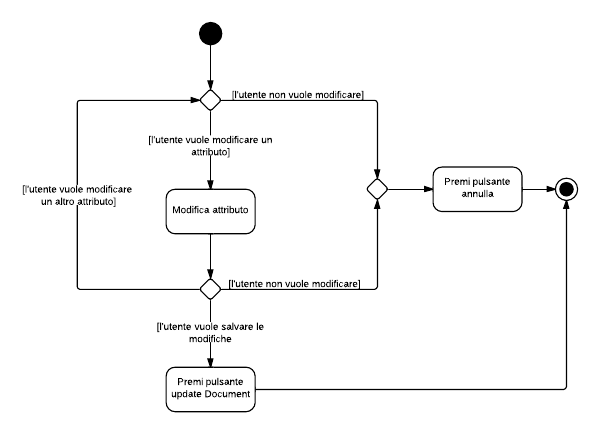
\includegraphics[scale=0.5]{uml/MaaP - Modifica document.png}
\caption{Diagramma di attività - Modifica del Document selezionato}
\end{figure}

L'utente con privilegi di scrittura può modificare ogni singolo attributo del \glossario{Document} selezionato, editando i rispettivi campi di testo. Una volta che ha terminato le modifiche preme il pulsante di \textit{update}; il sistema \glossario{MaaP} verificherà che le modifiche apportate siano corrette e rispettino i vincoli del \glossario{database}. In ogni momento l'utente può comunque decidere di annullare le modifiche e tornare alla pagina precedente.

\subsubsection{Apri pagina gestione utenti}

\begin{figure}[H]
\centering
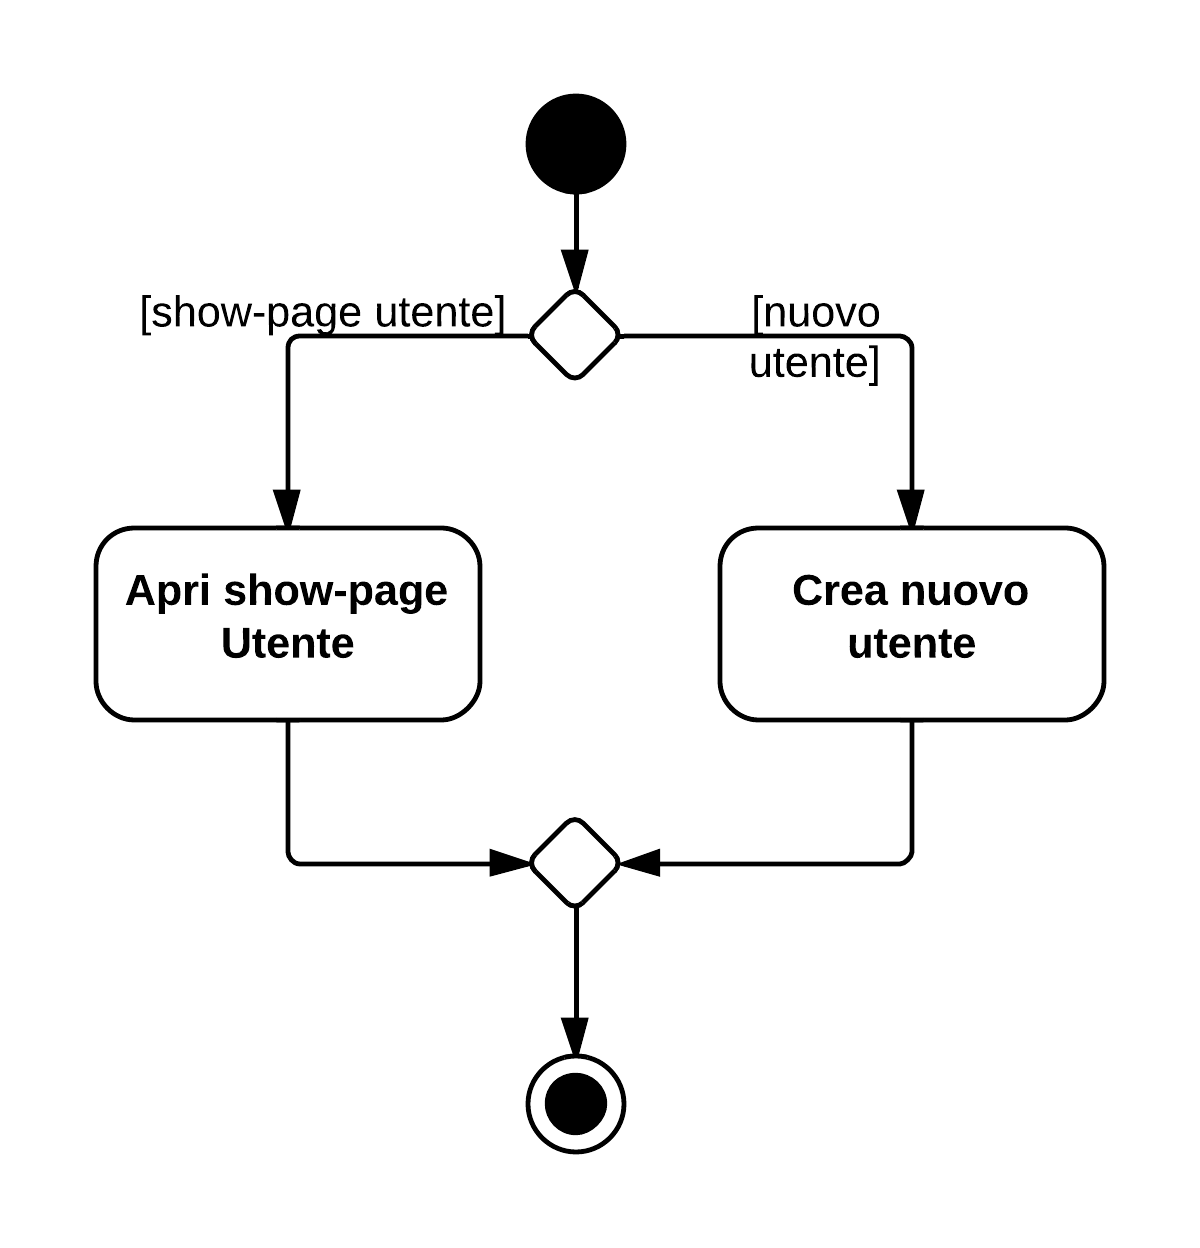
\includegraphics[scale=0.3]{uml/MaaP - Apri pagina gestione utenti.png}
\caption{Diagramma di attività - Pagina di gestione degli utenti}
\end{figure}

Un admin dell'applicazione può accedere a una pagina in cui poter gestire gli utenti. Essa consiste fondamentalmente in una \glossario{index-page} contenente la lista di tutti gli utenti presenti nel sistema. L'admin può da questa pagina selezionare un utente, e visualizzare quindi la sua relativa \glossario{show-page}, o crearne uno nuovo aprendo la pagina di creazione.

\subsubsection{Apri show-page utente}

\begin{figure}[H]
\centering
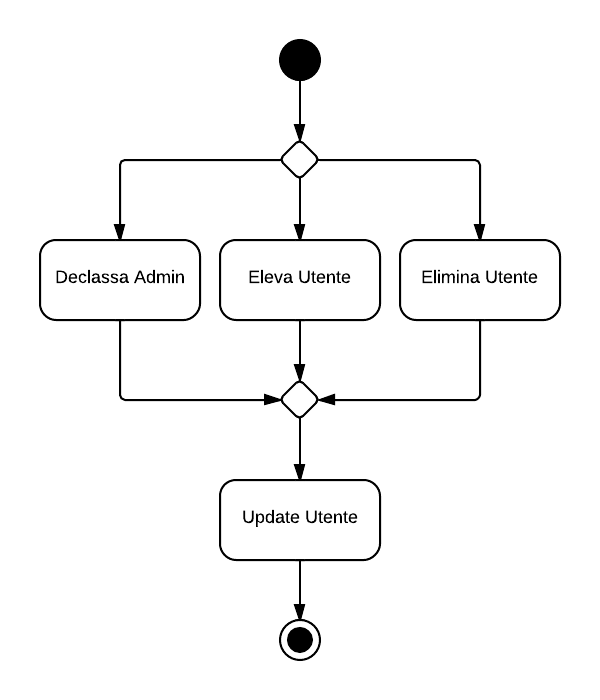
\includegraphics[scale=0.4]{uml/MaaP - Apri show-page utente.png}
\caption{Diagramma di attività - Pagina di visualizzazione di un utente}
\end{figure}

In questa pagina l'admin visualizza la \glossario{show-page} dell'utente selezionato e può compiere le seguenti operazioni:

\begin{itemize}

	\item Se l'utente selezionato è un admin può declassarlo e portarlo a livello di utente normale. Naturalmente non può declassare se stesso e il \textit{super-admin}, in modo da far sì che in qualsiasi momento sia presente almeno un admin nel sistema;
	\item Se l'utente non è un admin può elevarlo da utente normale a livello di admin;
	\item Eliminare l'utente selezionato dal sistema.

\end{itemize}

Il sistema \glossario{MaaP} si occuperò di apportare tutte le modifiche effettuate dall'admin al \glossario{database} delle credenziali.

\subsubsection{Crea un nuovo utente}

\begin{figure}[H]
\centering
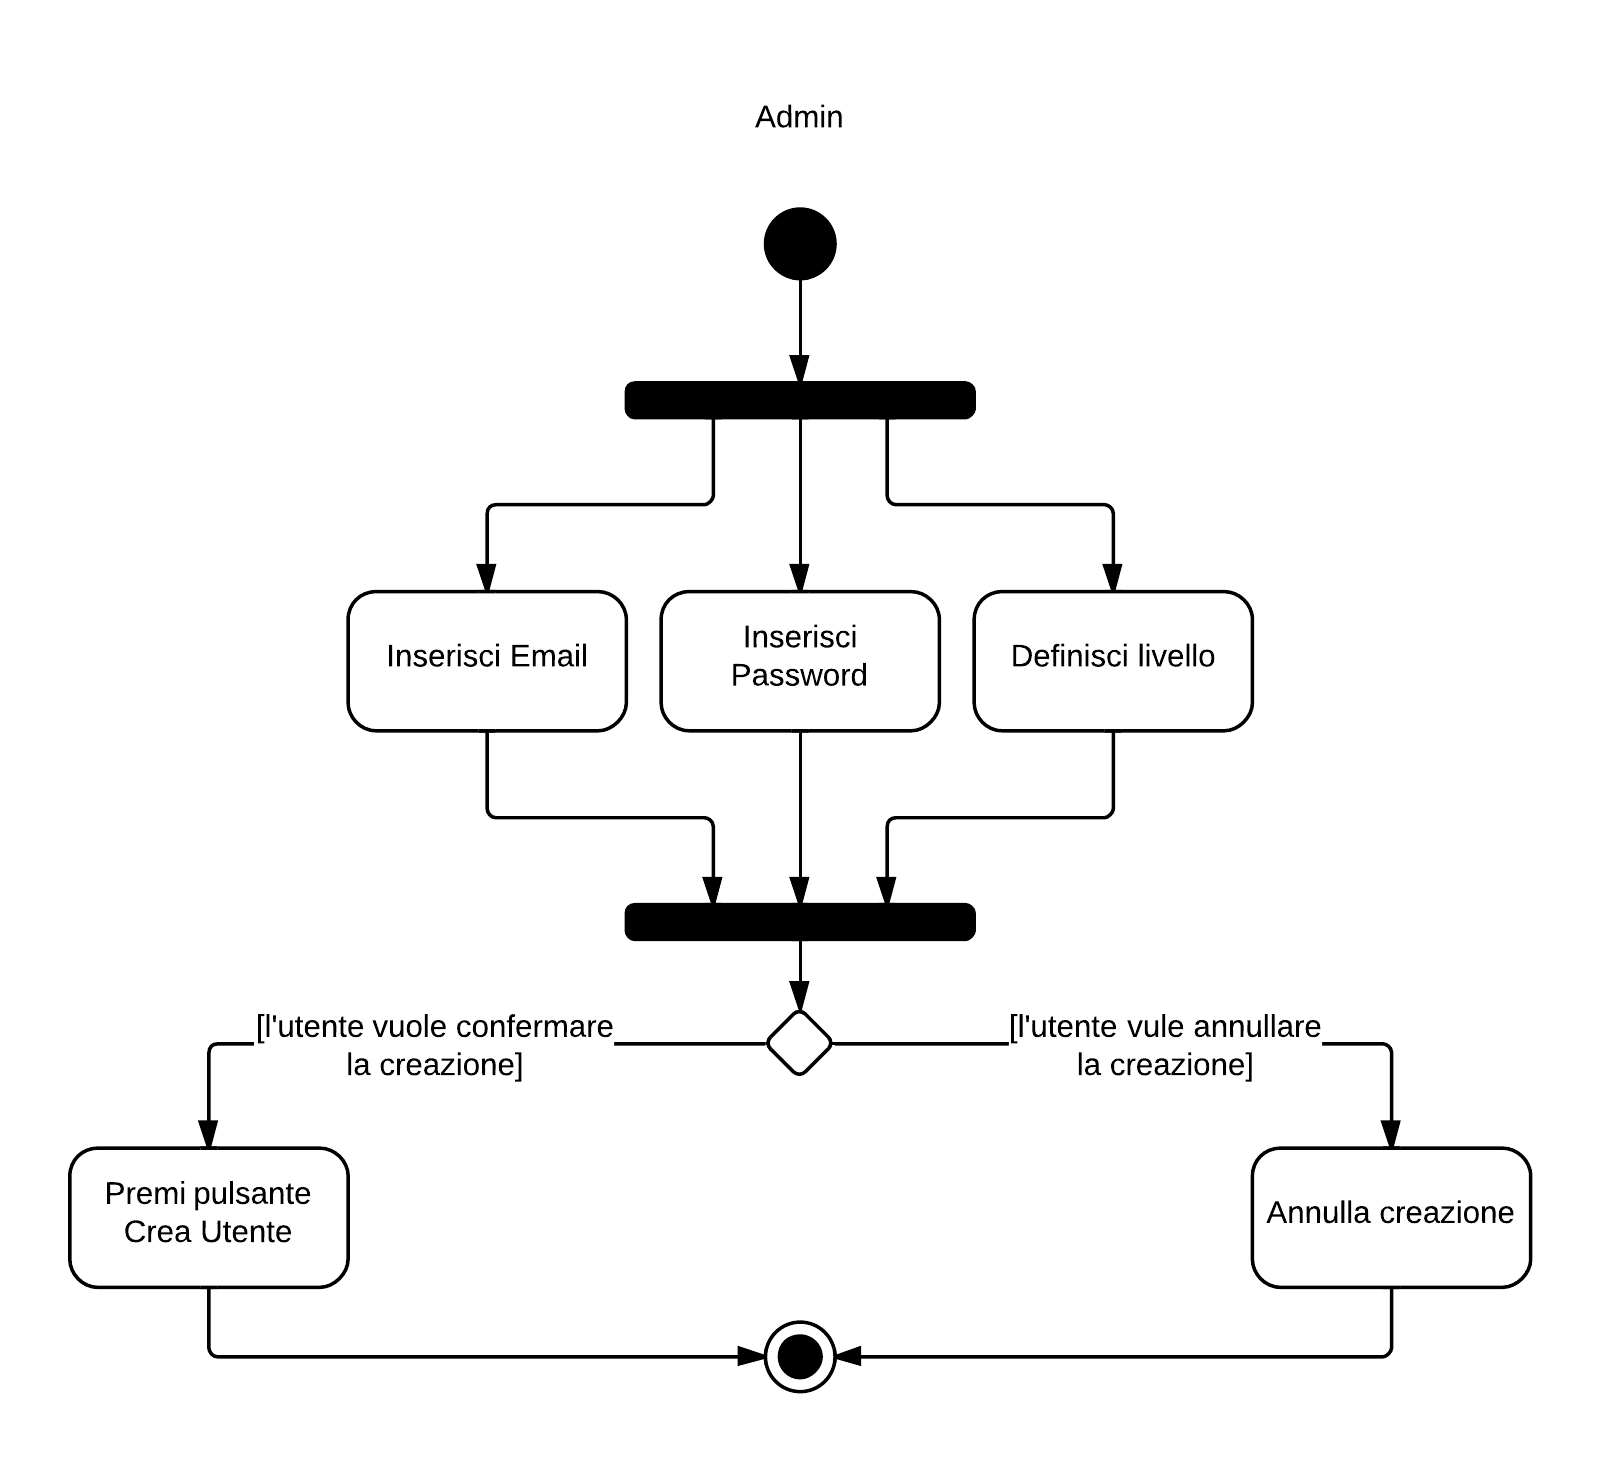
\includegraphics[scale=0.4]{uml/MaaP - Crea nuovo utente.png}
\caption{Diagramma di attività - Pagina di creazione di un nuovo utente}
\end{figure}

L'admin entra in un'apposita pagina di creazione di un nuovo utente e al suo interno può definire:

\begin{itemize}

	\item L'indirizzo email del nuovo utente;
	\item La password del nuovo utente;
	\item Il livello del nuovo utente, che potrà essere o utente normale o admin;

\end{itemize}

Una volta completate le modifiche l'utente può decidere di confermare o annullare le modifiche, premendo i relativi pulsanti. Il sistema \glossario{MaaP}, nel caso in cui l'utente abbia deciso di confermare le modifiche, si occuperà di inserire nel \glossario{database} delle credenziali il nuovo utente creato.

\subsection{Servizio MaaS}

Vengono di seguito descritte tutte le iterazioni che un utente può effettuare con il servizio web \glossario{MaaS}.

\subsubsection{Attività principali}

\begin{figure}[H]
\centering
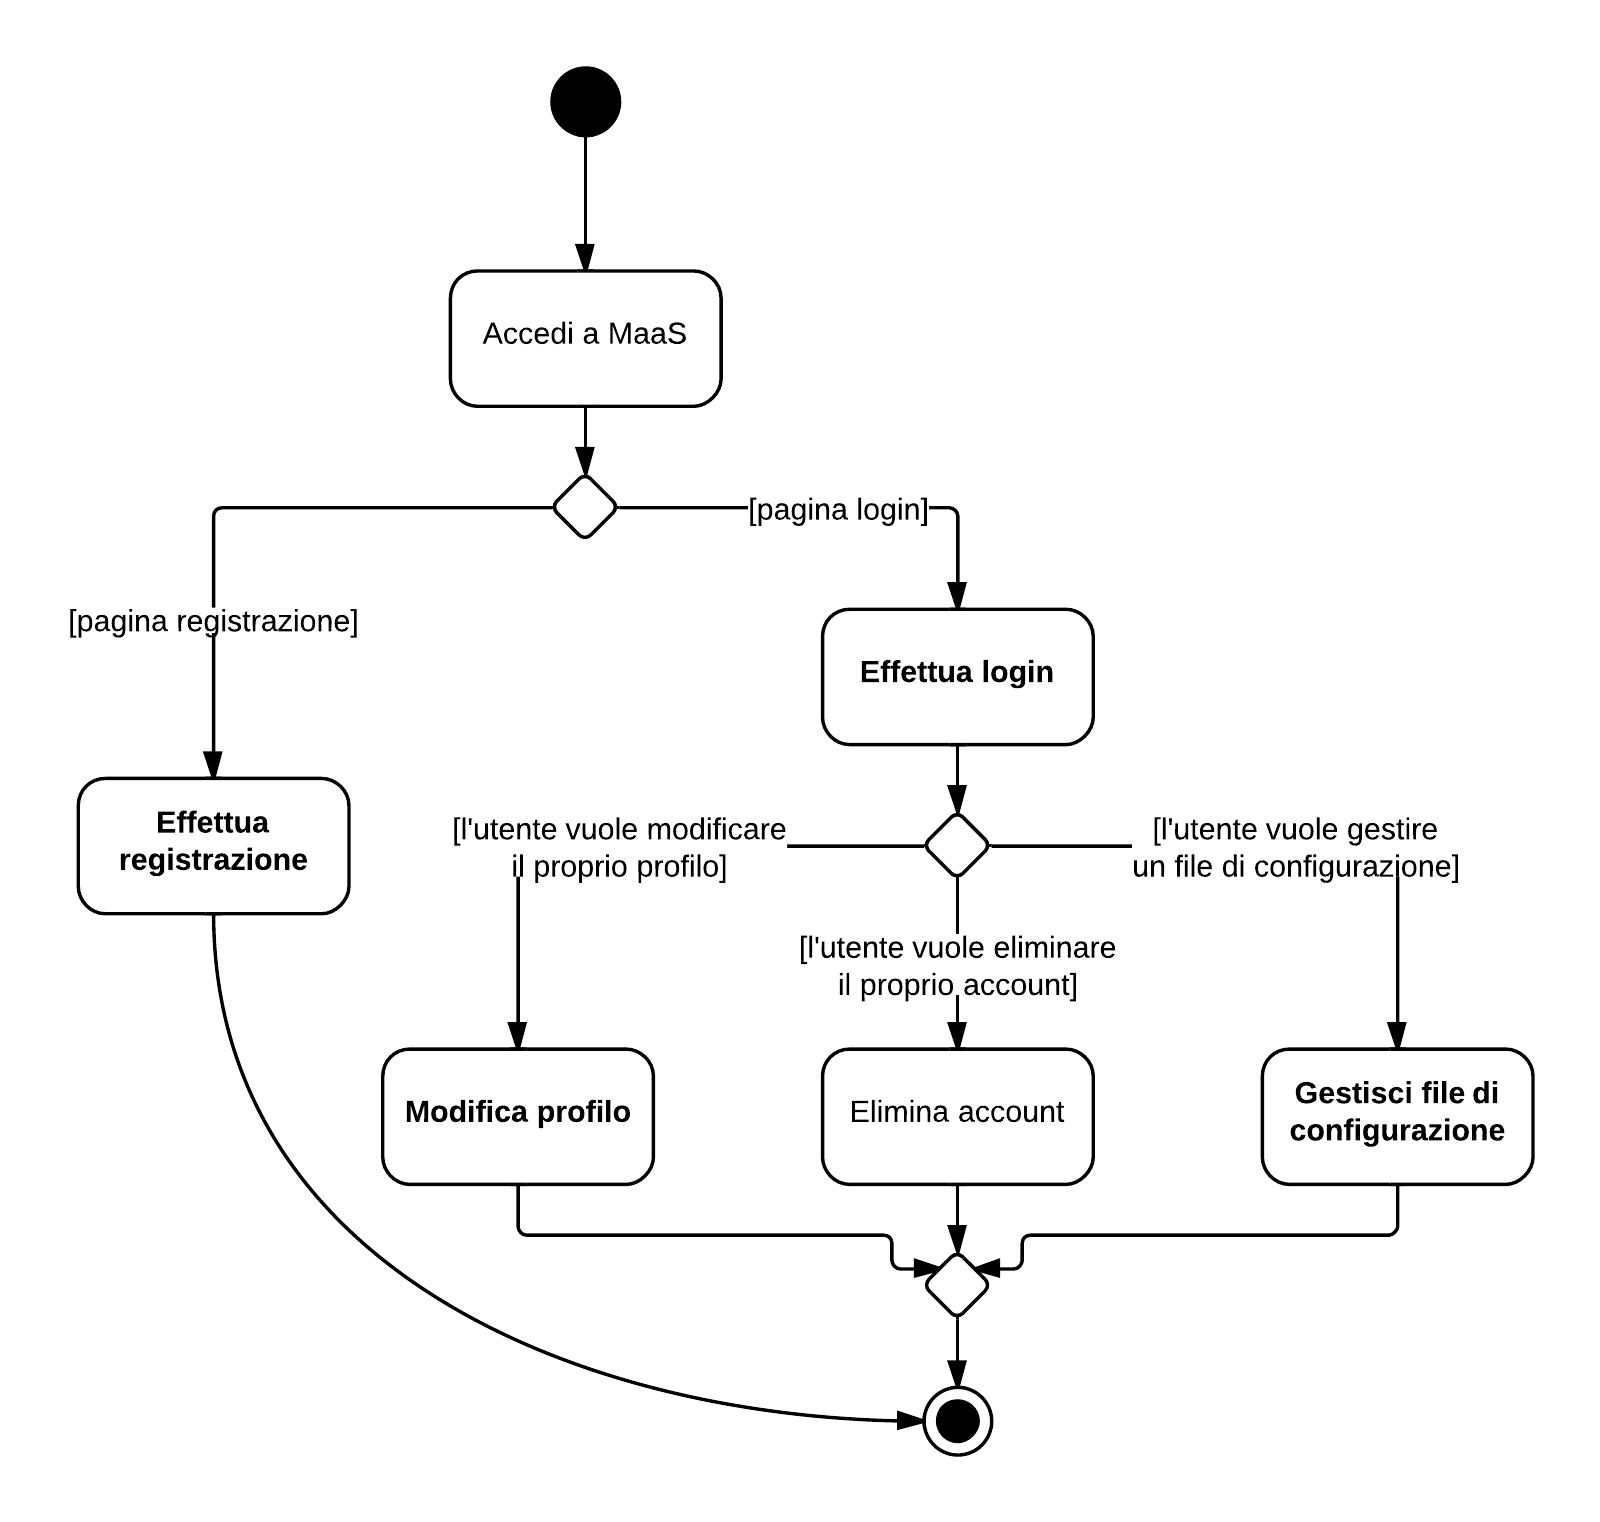
\includegraphics[scale=0.7]{uml/MaaS - Attivita principali.png}
\caption{Diagramma di attività - Attività principali di MaaS}
\end{figure}

% TODO descrizione

\subsubsection{Effettua registrazione}

\begin{figure}[H]
\centering
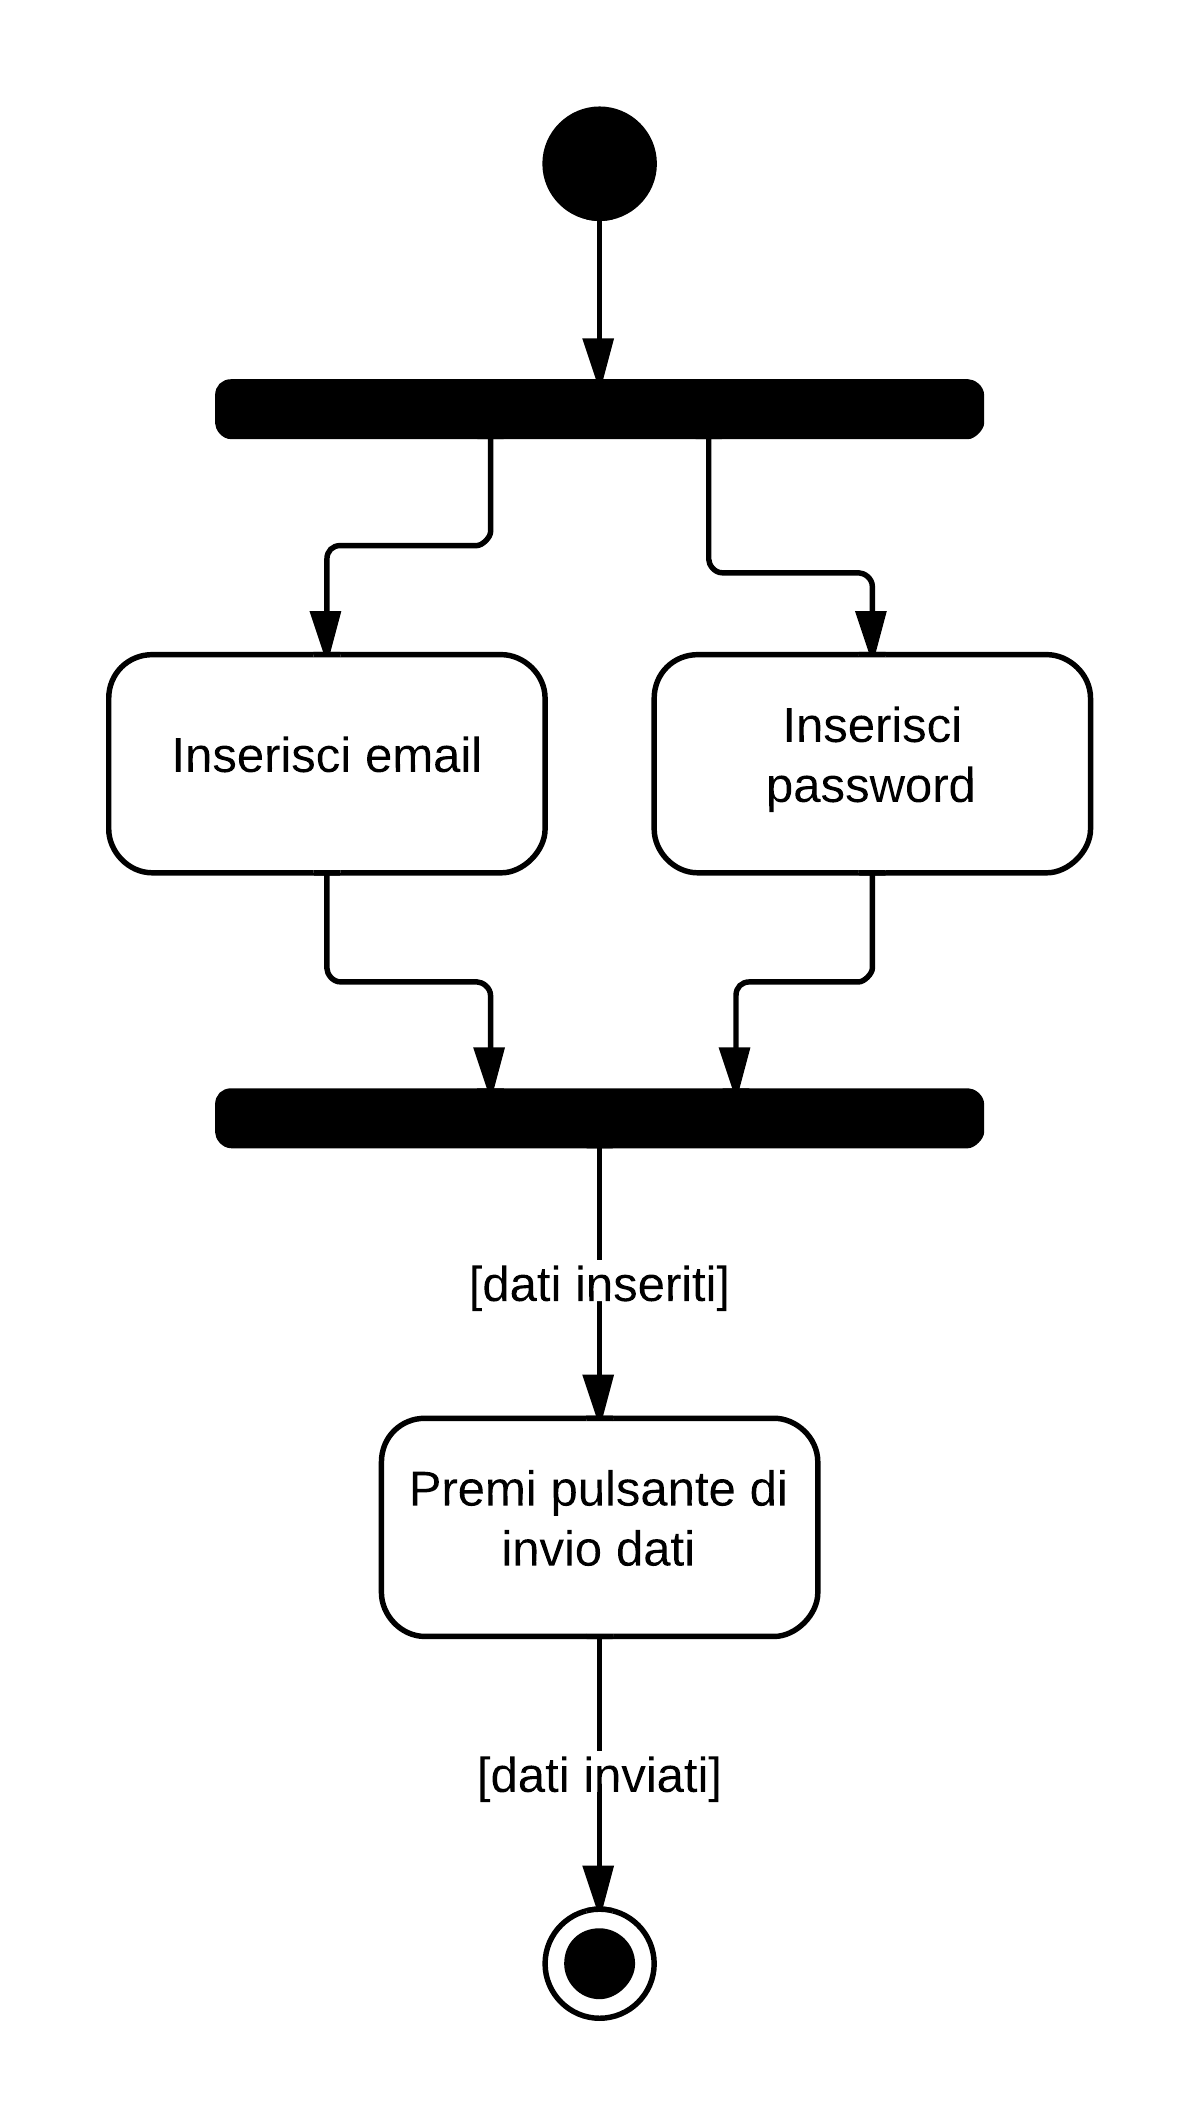
\includegraphics[scale=0.7]{uml/MaaP - Effettua registrazione.png}
\caption{Diagramma di attività - Registrazione al servizio MaaS}
\end{figure}

% TODO descrizione

\subsubsection{Effettua login}

\begin{figure}[H]
\centering
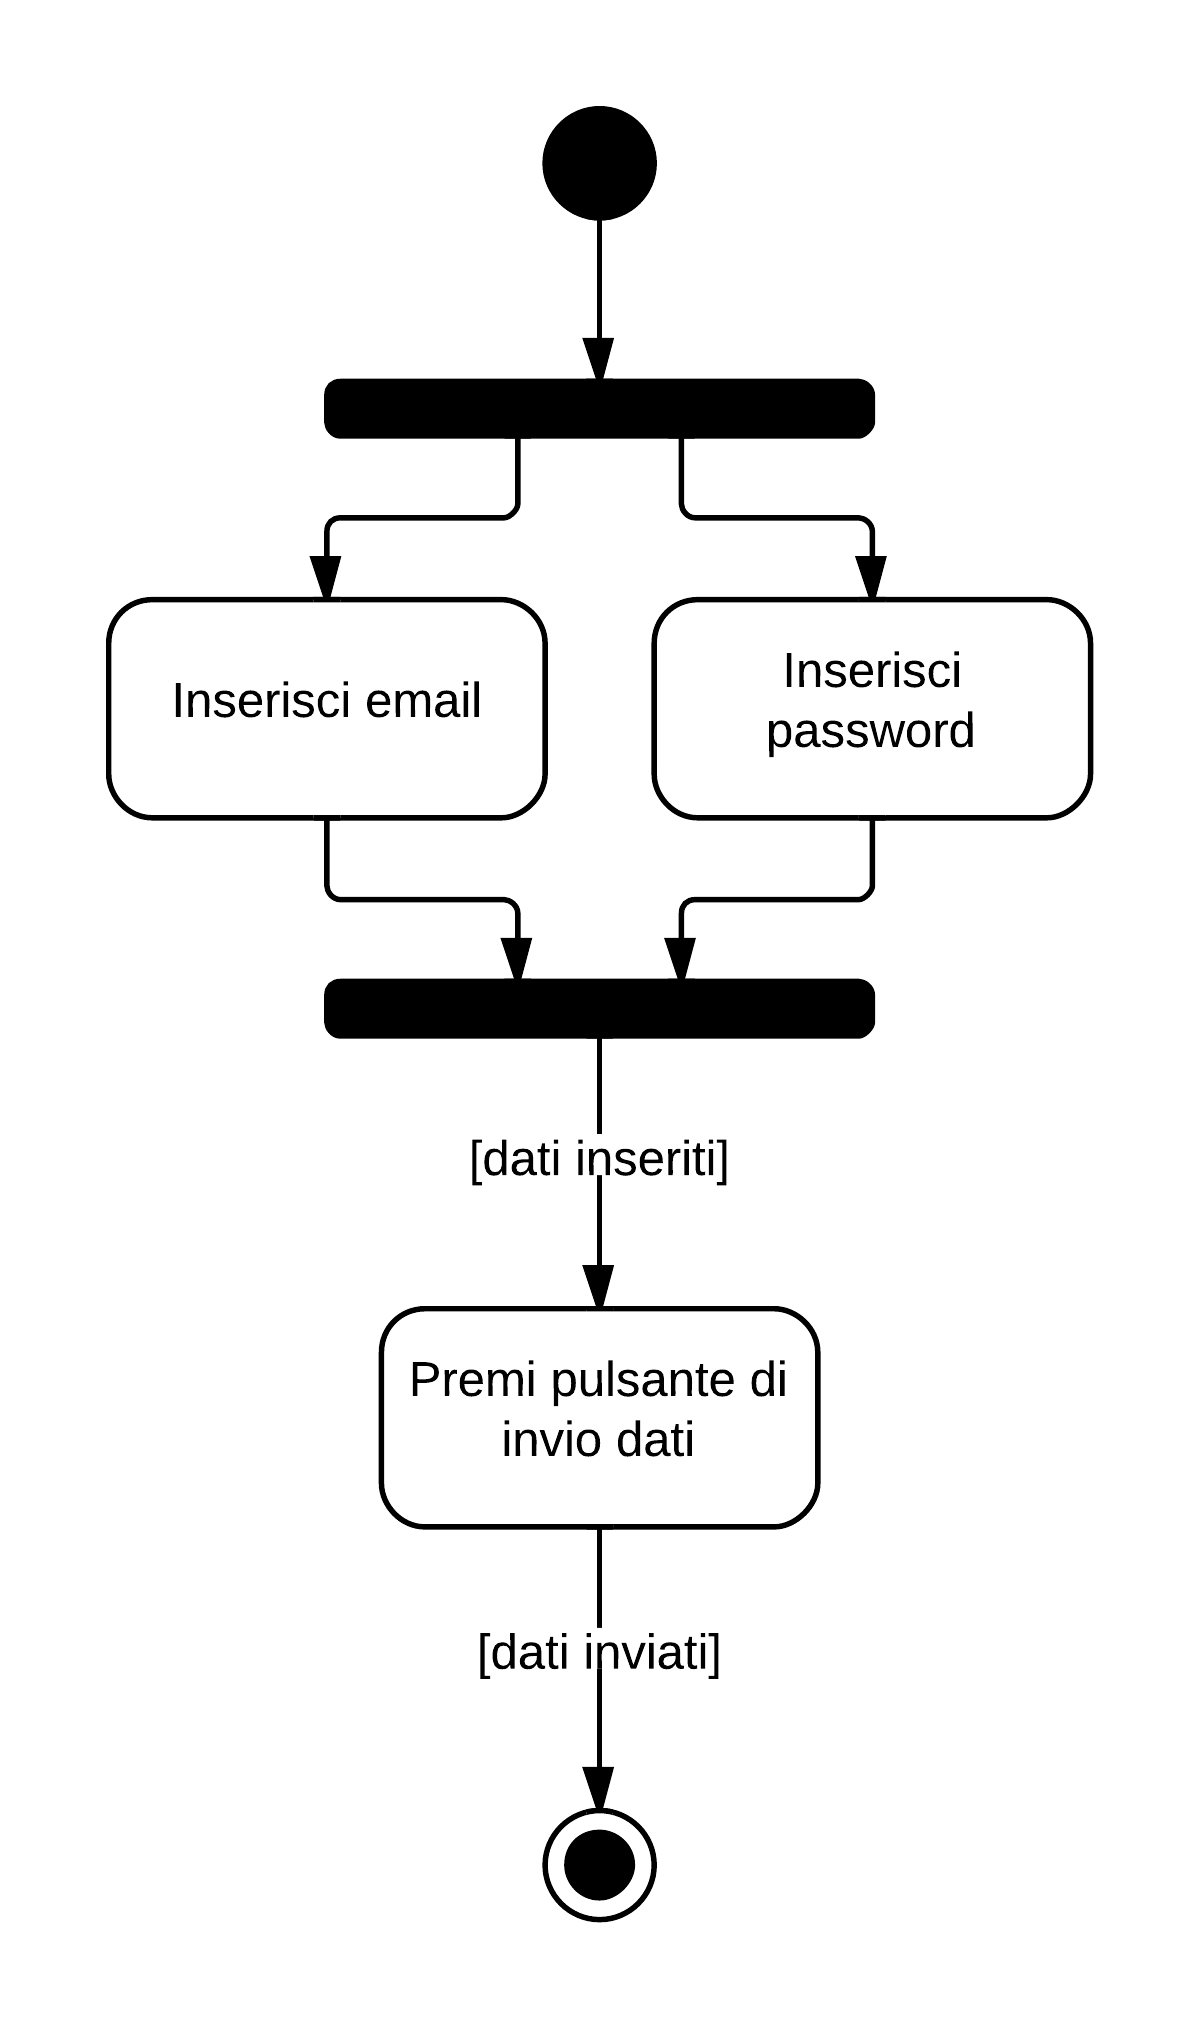
\includegraphics[scale=0.7]{uml/MaaP - Effettua login.png}
\caption{Diagramma di attività - Login al servizio MaaS}
\end{figure}

% TODO descrizione

\subsubsection{Modifica profilo}

%\begin{figure}[H]
%\centering
%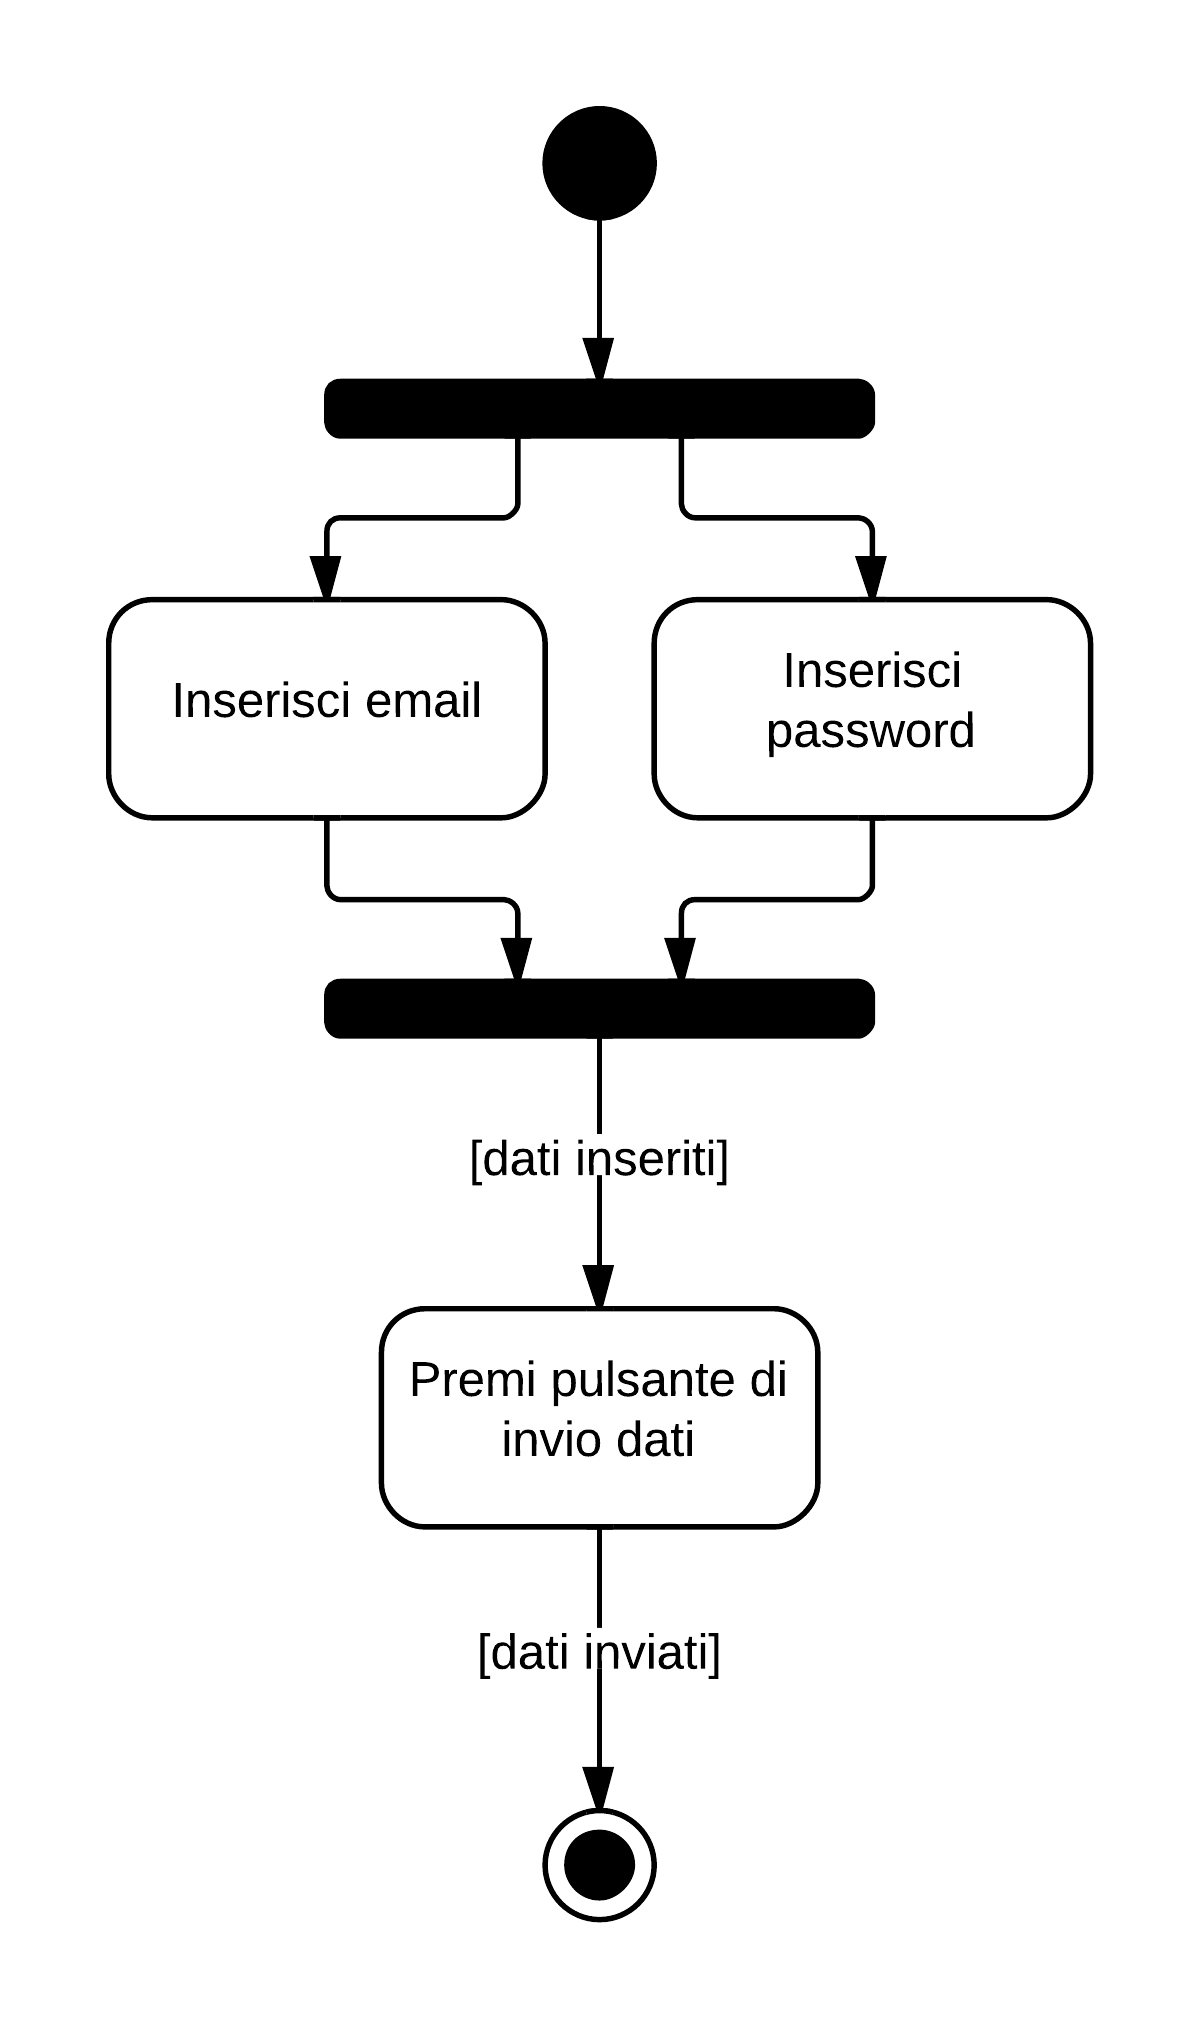
\includegraphics[scale=0.7]{uml/MaaP - Effettua login.png}
%\caption{Diagramma di attività - Login al servizio MaaS}
%\end{figure}
